\chapter{CLI Reference (Practical)}

\ChapterMeta{
This chapter provides a concise summary of the most frequently utilized commands and demonstrates how to explore the complete Command Line Interface (CLI) surface via the \cmd{--help} flag.
}{
It is designed to minimize the time to first execution and to clearly delineate which commands are install-safe versus those restricted to repository-only workflows.
}{
Utilize \cmd{yolozu --help} for the pip-installed CLI, or \cmd{python3 tools/yolozu.py --help} for the repository wrapper. Because implementation details evolve, the \cmd{--help} output remains the definitive source of truth.
}
\ChapterAudience{Read this chapter when you want copy-paste entrypoints first and detailed tool discovery second.}


\section{Design Philosophy}
The CLI surface is intentionally bifurcated to serve distinct user profiles:
\begin{itemize}
  \item \cmd{yolozu}: The end-user safe CLI, installed globally or virtually via pip.
  \item \cmd{python3 tools/yolozu.py}: The repository wrapper, specifically tailored for research and evaluation pipelines.
\end{itemize}

This chapter documents the \textit{high-traffic commands} and outlines the methodology for discovering the broader command set.

\section{Discoverability}
As a best practice, always initiate discovery with:\\
\cmd{yolozu --help} and \cmd{yolozu <command> --help}.\\
For repository-specific workflows, utilize: \cmd{python3 tools/yolozu.py --help}.

\section{Common Commands}
\begin{longtable}{@{}p{0.40\textwidth}p{0.55\textwidth}@{}}
\toprule
\textbf{Command} & \textbf{Purpose} \\
\midrule
\cmd{yolozu doctor} & Executes environment diagnostics (verifying dependencies, GPU status, and backend availability). \\
\cmd{yolozu completion} & Prints shell completion scripts (\cmd{--shell bash|zsh}) for interactive command completion. \\
\cmd{yolozu demo overview} & Writes a demo overview report (\path{demo\_output/overview/...}) covering bbox/segmentation/keypoints/depth/pose6d flows, dependency checks, and recommended commands. \\
\cmd{yolozu demo} & Runs a small CPU-friendly demo suite and writes artifacts under \path{demo\_output/}. \\
\cmd{yolozu demo instance-seg} & Instance-seg demo (offline by default). \newline
For real-image overlays: \cmd{--background yolo-bbox --yolo-root data/smoke --yolo-split val --inference none}. \newline
For polygon masks/inference: \cmd{--background coco-instances}. \\
\cmd{yolozu demo instance-seg-tta} & Real-image instance-seg TTA compare demo. Scans a small COCO polygon subset, applies a deterministic corruption, then writes raw-vs-augmentation-based-TTA overlays under \path{demo\_output/instance\_seg\_tta/} or the chosen \cmd{--run-dir}. \\
\cmd{yolozu demo keypoints} & Keypoint R-CNN inference demo (torchvision; writes overlay under \path{demo\_output/keypoints/}). \\
\cmd{yolozu demo pose} & 6D pose demo (chessboard/ArUco by default; ArUco sample cached under \path{demo\_output/pose/\_samples/}; DenseFusion requires CUDA + large downloads). Writes overlay under \path{demo\_output/pose/}. \\
\cmd{yolozu demo depth} & Monocular depth inference demo (default: Depth Anything via Transformers; optional MiDaS/DPT; writes images under \path{demo\_output/depth/}). \\
\cmd{yolozu demo train} & Training demo (MNIST fine-tune; bounded by \cmd{--max-steps}; downloads ResNet18 on first run; writes under \path{demo\_output/train/}). \\
\cmd{yolozu demo continual} & Continual-learning demo (toy synthetic by default; \cmd{--problem mnist\_rotate} uses a vision backbone). \\
\cmd{yolozu list models} & Lists curated model IDs available for reproducible downloads. \\
\cmd{yolozu fetch <model\_id> --accept-license} & Downloads a model artifact with cache reuse, sha256 verification, and license gating; records \path{models/<id>/meta.json}. (Custom registries may require \cmd{--allow-unsafe} / \cmd{--allow-non-apache}.) \\
\cmd{bash scripts/smoke.sh} & Runs the one-command offline smoke flow (doctor + validate + eval-coco dry-run + SynthGen intake smoke + instance-seg overlay PNG evidence on \path{data/smoke}). \\
\cmd{bash scripts/smoke.sh --profile deep} & Runs the deep walkthrough profile and writes \path{reports/smoke\_walkthrough\_report.json} plus backend dry-run export artifacts. \\
\cmd{bash scripts/smoke.sh --help} & Shows smoke CLI options (\cmd{--dataset}, \cmd{--predictions}, \cmd{--report}, \cmd{--synthgen-root}, \cmd{--synthgen-predictions}, \cmd{--output-dir}, \cmd{--demo-run-dir}, \cmd{--skip-demo}, \cmd{--torch-device}, \cmd{--profile}, \cmd{--walkthrough-report}). \\
\cmd{bash scripts/ttt\_compare.sh} & Short baseline-vs-adapted TTT compare wrapper. Use \cmd{--boilerplate tent|mim|mim\_probe|cotta|eata|sar} plus \cmd{--dataset}, \cmd{--checkpoint}, and \cmd{--run-dir}; it writes baseline/adapted predictions and a before-after Markdown+JSON summary. \\
\cmd{yolozu train} & Initiates YAML/JSON config-driven RT-DETR training (fully supporting the run contract and resumption capabilities). \\
\cmd{yolozu test} & Executes the YAML/JSON scenario runner (compatible with dummy, precomputed, and rtdetr\_pose adapters). \\
\cmd{yolozu predict-images} & Performs folder-level inference, generating predictions, visual overlays, and an HTML summary. \\
\cmd{yolozu eval-coco} & Conducts COCO mAP evaluation derived from \path{predictions.json} (requires COCO tooling to be installed). \\
\cmd{yolozu benchmark} & Parity-target benchmark entrypoint. Runs real backend orchestration for \cmd{torch}/\cmd{onnx}/\cmd{engine} when artifacts and runtimes exist, otherwise records explicit skipped/placeholder results. Key knobs include \cmd{--protocol}, backend-specific model overrides (\cmd{--torch-model}, \cmd{--onnx-model}, \cmd{--engine-model}), and \cmd{--latency-source auto}. \\
\cmd{yolozu parity} & Compares two distinct predictions artifacts to detect backend drift or discrepancies. \\
\cmd{yolozu predictions migrate} & Migrates predictions entry schema versions (currently \cmd{--from v1 --to v2}) with optional strict source checking. \\
\cmd{yolozu calibrate} & Applies score calibration and long-tail post-hoc adjustments. \\
\cmd{yolozu long-tail-recipe} & Generates a long-tail training recipe JSON with selectable sampler/loss/metric/lr scheduler plugins. \\
\cmd{python3 tools/eval_suite.py} & Executes suite evaluation, providing protocol-pinned reporting and cross-run comparisons. \\
\cmd{python3 tools/run\_reference\_adapter\_regression.py} & Runs RT-DETR reference-adapter regression with profile-aware micro/full modes, interface contract gates (hard), behavior/parity gates (warn/hard), deterministic-preprocess metadata checks, provenance snapshot capture (\cmd{--capture-provenance}), matrix baseline layout (\cmd{--baseline-layout matrix}), lock/hash enforcement, and failure artifacts (\cmd{--diff-summary-out}, \cmd{--topk-examples-dir}). \\
\cmd{python3 tools/hpo_sweep.py} & Orchestrates hyperparameter sweeps and aggregates metrics into CSV, MD, or JSONL formats. \\
\cmd{python3 tools/benchmark\_model.py} & Repository wrapper for \cmd{yolozu benchmark}; useful when backend-specific benchmark behavior must also be tracked in \path{tools/manifest.json}. \\
\cmd{python3 tools/run\_ttt\_compare.py} & Python entrypoint for the same TTT compare workflow; loads method boilerplates from \path{configs/examples/ttt\_compare/} and writes `plan.json`, before/after predictions, optional eval reports, and compare summaries. \\
\cmd{python3 tools/render\_ttt\_manual\_figures.py} & Renders the checked-in TTT summary/workflow/qualitative PNG figures from fixed report artifacts for \path{docs/assets/} and \path{manual/figures/}. \\
\cmd{python3 tools/benchmark_latency.py} & Runs the latency/FPS benchmark harness, maintaining a JSONL history to track performance regressions. \\
\cmd{python3 tools/check\_repo\_governance.py} & Audits local governance evidence plus exported GitHub settings snapshots for branch protection, review policy, and repository-security posture. Writes a JSON summary and keeps history-based items explicit instead of pretending they are source-only facts. \\
\cmd{python3 tools/validate_tool_manifest.py} & Validates the structural integrity of the machine-readable registry (\path{tools/manifest.json}). \\
\cmd{bash release.sh} & Runs no-option release automation: auto SemVer/CalVer version bump policy, tag push, GitHub release publish, and PyPI/Zenodo workflow handoff. \\
\cmd{python3 tools/support\_yolo\_detr.py} & YOLO/DETR support utility with fixed 3-layer interface contract (trainer/repo/export), short aliases (\cmd{ls/tu/th/eo/pn}), preset defaults (\cmd{-P smoke}), shared dataset conversion, ONNX export templates, and prediction canonicalization. \\
\bottomrule
\end{longtable}

\section{Demo Output Examples (Images)}
The \cmd{yolozu demo *} commands are designed to produce concrete artifacts (JSON reports and overlay images)
that help users verify they can run end-to-end workflows.

The figures below are committed snapshots generated from \path{data/smoke} using the following commands:
\begin{lstlisting}[language=bash]
yolozu demo instance-seg \
  --background yolo-bbox --yolo-root data/smoke --yolo-split val --inference none \
  --num-images 1 --image-size 320 --max-instances 3 \
  --run-dir demo_output/manual/instance_seg

yolozu demo keypoints \
  --image data/smoke/images/val/000000000036.jpg --device cpu --max-persons 1 \
  --run-dir demo_output/manual/keypoints

yolozu demo depth \
  --image data/smoke/images/val/000000000036.jpg --device cpu --model midas_small \
  --run-dir demo_output/manual/depth

yolozu demo pose \
  --backend chessboard --sample-source synthetic \
  --run-dir demo_output/manual/pose
\end{lstlisting}

\begin{figure}[htbp]
  \centering
  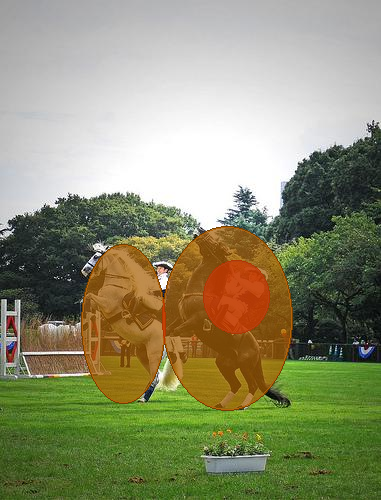
\includegraphics[width=0.95\textwidth]{figures/demo_instance_seg_overlay.png}
  \caption{Instance-seg demo overlay (\cmd{--background yolo-bbox --inference none}). This offline mode uses GT-derived scaffold predictions for visualization and evaluation smoke checks.}
\end{figure}

\begin{figure}[htbp]
  \centering
  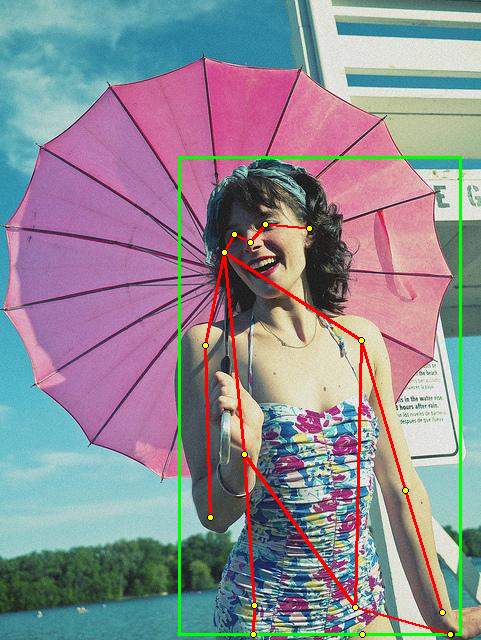
\includegraphics[width=0.95\textwidth]{figures/demo_keypoints_overlay.png}
  \caption{Keypoints demo overlay (torchvision Keypoint R-CNN).}
\end{figure}

\begin{figure}[htbp]
  \centering
  
\includegraphics[width=0.95\textwidth]{figures/demo_depth_overlay.png}
  \caption{Depth demo overlay (MiDaS small; relative depth visualization).}
\end{figure}

\begin{figure}[htbp]
  \centering
  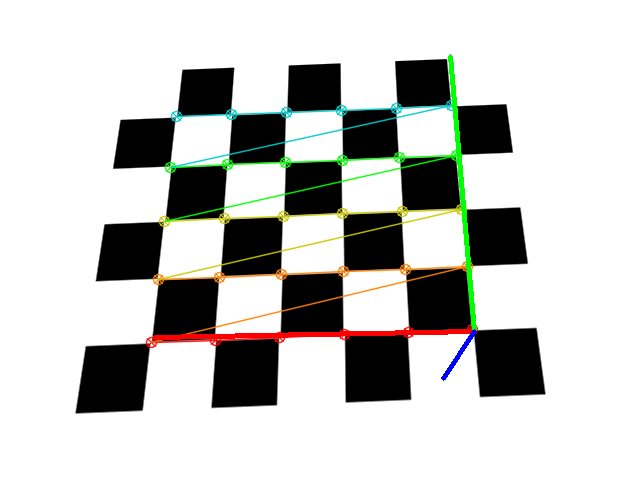
\includegraphics[width=0.95\textwidth]{figures/demo_pose_overlay.png}
  \caption{Pose6D demo overlay (chessboard + OpenCV solvePnP).}
\end{figure}

\subsection{Long-tail recipe plugin options (PyTorch)}
\cmd{yolozu long-tail-recipe} supports explicit plugin choices for loss, validation metric, and learning-rate scheduler.

\begin{lstlisting}[language=bash]
yolozu long-tail-recipe \
  --dataset data/smoke --split val \
  --loss-plugin torch_cross_entropy \
  --metric-plugin torch_top1_accuracy \
  --lr-scheduler torch_step_lr \
  --output reports/long_tail_recipe_torch.json --force
\end{lstlisting}

Primary plugin flags:
\begin{itemize}
  \item \cmd{--loss-plugin}: \cmd{none}, \cmd{focal}, \cmd{ldam}, \cmd{torch\_cross\_entropy}, \cmd{torch\_nll\_loss}, \cmd{torch\_bce\_with\_logits}
  \item \cmd{--metric-plugin}: \cmd{none}, \cmd{torch\_top1\_accuracy}, \cmd{torch\_top5\_accuracy}, \cmd{torch\_cross\_entropy}
  \item \cmd{--lr-scheduler}: \cmd{none}, \cmd{torch\_step\_lr}, \cmd{torch\_cosine\_annealing\_lr}, \cmd{torch\_reduce\_on\_plateau}, \cmd{torch\_one\_cycle\_lr}
\end{itemize}

\section{YAML Config-Driven Usage (Train/Test/Resume)}
\yolozu{} supports the ingestion of a YAML or JSON configuration file as its primary positional argument.
Internally, \cmd{yolozu train} delegates the \cmd{--config <file>} argument to \path{rtdetr_pose.train_minimal}, whereas \cmd{yolozu test} maps YAML keys directly to \path{yolozu.scenarios_cli} arguments.

\begin{longtable}{@{}p{0.18\textwidth}p{0.30\textwidth}p{0.46\textwidth}@{}}
\toprule
\textbf{Use Case} & \textbf{YAML File} & \textbf{Command Pattern} \\
\midrule
Train (Default) & \path{configs/examples/train_setting.yaml} & \cmd{yolozu train <train_setting.yaml>} \\
Train (Contract) & \path{configs/examples/train_contract.yaml} & \cmd{yolozu train <train_contract.yaml> --run-id <id>} \\
Resume & Same as Train (Contract) & \cmd{yolozu train <train_contract.yaml> --run-id <id> --resume} \\
Test (Scenario) & \path{configs/examples/test_setting.yaml} & \cmd{yolozu test <test_setting.yaml> [test_args...]} \\
\bottomrule
\end{longtable}

Concrete execution examples:
\begin{lstlisting}[language=bash]
yolozu train configs/examples/train_setting.yaml
yolozu train configs/examples/train_contract.yaml --run-id exp01
yolozu train configs/examples/train_contract.yaml --run-id exp01 --resume
yolozu test configs/examples/test_setting.yaml --adapter precomputed --predictions reports/predictions.json
\end{lstlisting}

Backbone substitutions are governed exclusively by the model configuration JSON, rather than by modifying adapter commands directly:
\begin{lstlisting}[language=bash]
yolozu train configs/examples/train_setting.yaml \
  --model-config rtdetr_pose/configs/base.json
\end{lstlisting}

For comprehensive details regarding the backbone contract and supported architectures, refer to \path{docs/backbones.md}.

\subsection{Test YAML and the Override Rule}
The default test YAML configuration is intentionally minimalist (typically specifying only the adapter, dataset, split, and max\_images). Runtime-specific parameters are conventionally supplied as CLI overrides:
\begin{lstlisting}[language=bash]
yolozu test configs/examples/test_setting.yaml \
  --adapter rtdetr_pose \
  --config rtdetr_pose/configs/base.json \
  --checkpoint /path/to/checkpoint.pt \
  --dataset data/smoke \
  --max-images 50
\end{lstlisting}

\noindent This paradigm directly mirrors the documented real-model workflow detailed in \path{docs/real_model_interface.md}.

\section{Repository Power Tools}
A multitude of task-specific scripts are housed within the \path{tools/} directory. Notable examples include:
\begin{itemize}
  \item \path{tools/validate_predictions.py}
  \item \path{tools/eval_instance_segmentation.py}
  \item \path{tools/eval_segmentation.py}
  \item \path{tools/export_predictions.py} (Facilitates adapter-based export)
\end{itemize}

For an exhaustive inventory, consult \path{tools/manifest.json} (for machine-readable metadata) and the documentation index (for human-readable guidance).
